\section{Woebot}
Woebot is an intelligent software agent for mental health.
It is powered by an artificial intelligence and natural language processing.
With the help of different therapeutic approaches it should help patients overcome their problems and support them with their mental health.
Although Woebot appears to be a mental health service, the terms of service state that this is not the case\cite{woebot-tos}.
Woebot is designed to be a pure self-help program.
It is available for smartphones on Google Play or the App Store\cite{woebot-download}.
There are several versions of Woebot which are currently in clinical trials or research.
This study only focuses on the non-prescription version for adult mental health.
It is advertised as a tool that helps to monitor and managing symptoms of stress, depression and anxiety\cite{woebot-organizations}.
This tool comes with a variety of features.
This paper will briefly describe these features. \\

% Settings
The first thing that has to be done is creating and setting up an account.
After that a disclaimer states that Woebot is not a crisis service and no human will monitor the conversations between the user and the chatbot.
The generated data from conversations will also be anonymized. \\

\begin{figure}[ht]
  \begin{center}
    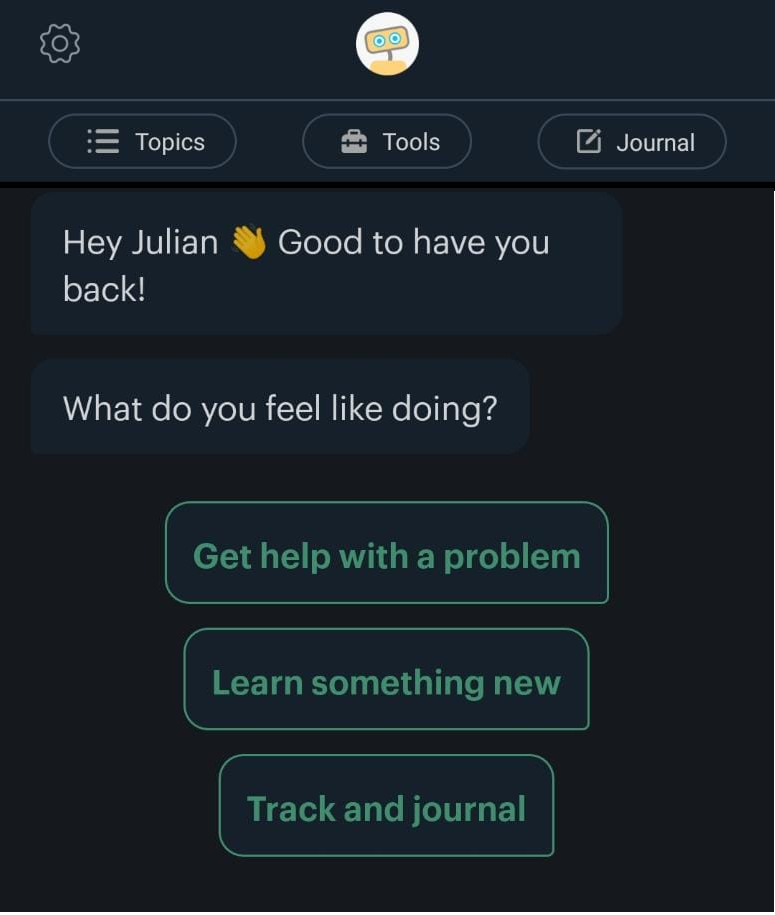
\includegraphics[width=1\columnwidth]{files/fullview.png}
    \caption{\label{fig:fullview} Cropped screenshot of the application}
  \end{center}
\end{figure}

The screenshot in \autoref{fig:fullview} shows the different functionalities of the application.
The gear-icon can be pressed to access the settings of the application.
There it is possible to manage account settings, set up a biometric lock or lookup the terms of service, privacy policy or licenses.\\

% Chat
The main functionality of the application is the chat-like conversation with Woebot.
It is similar to a lot of different instant-messaging apps like WhatsApp or Telegram\cite{whatsapp, telegram}.
Messages from Woebot appear on the left side and messages from the user on the right side.
Most of the time the user has to answer with predefined answers.
Otherwise, it is also possible to write inside a free text field.
While the answers from the user can only contain text based messages, Woebot is able to send GIFs or YouTube videos\cite{youtube}.\\

% Topics
The Topics-button takes the user to a list of different lessons.
The categories for these lessons range from understanding how the mind works to coping with the pandemic or managing stress.
Most lessons range from two to five minutes.
Although there are some lessons that could take up to twelve minutes.
Starting a lesson starts a conversation with Woebot.
For example choosing the lesson "Breaking your cabin fever" from the "Coping with a pandemic" category leads Woebot suggesting that a routine helps keeping the users spirit up.
Woebot also suggests spending time with exciting activities.
During this conversation, various GIFs and a YouTube video are being sent to the user.
The video material contains a child and Kermit from the Sesame Street saying the alphabet. \\

% Tools
The Tools-button enables the user to select from a variety of tools that are unlocked during the conversation with the chatbot.
Each tool also belongs into a category and pressing one results in starting a conversation.
This process is similar to the offered lessons in the topics-menu. One example tool is "Muscle relaxation".
Using this tool starts another conversation. Woebot warns the user that different muscle groups will be demanded.
In the event that the user is injured or has limited mobility it is also possible to skip certain exercises.
Woebot then suggests a video called "Progressive Muscle Relaxation" containing the exercises.
After the use of a tool Woebot asks if the user feels \texttt{better}, \texttt{same} or \texttt{worse}.
Selecting \texttt{better} leads to a brief explanation for the user to understand how or why the tool works.
In this case the "Stress increases muscle tension in our bodies, and progressive muscle relaxation can help release some of that." (Woebot), which has been proven by several studies\cite{progressive-muscle, stress-pmr}.
If the user reacts with the neutral or negative response Woebot suggest further tools.\\

% Journal
The last function in the toolbar is the Journal-button.
This button opens up two functionalities that are used for reflection.
The first functionality is a Mood Tracker which can be seen in \autoref{fig:moodtracker}.
These moods are recorded in the chat or via the function just mentioned in the journal tab.
A graph is created based on the entered moods.
This graph features emoticons that represent the different moods.
From left to right the emotions are ecstatic, helpless, ashamed, numb, numb and overwhelmed.\\

\begin{figure}[ht]
  \begin{center}
    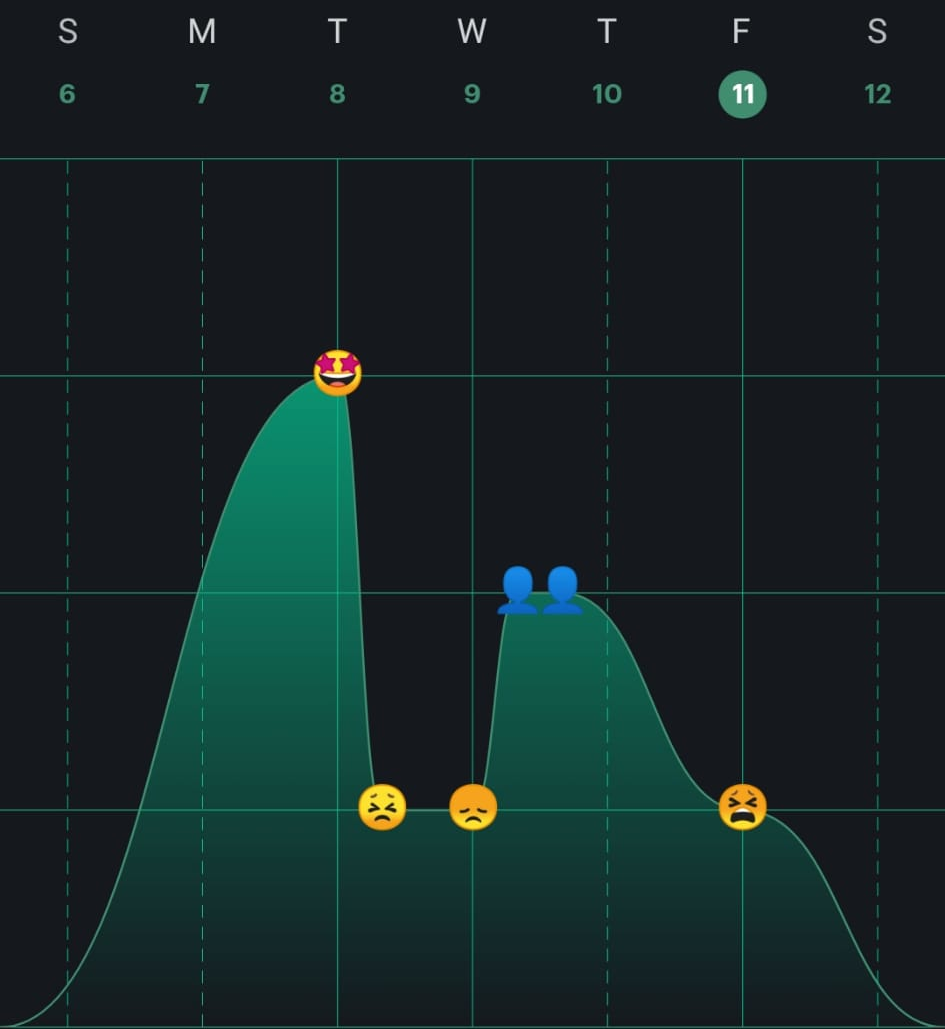
\includegraphics[width=1\columnwidth]{files/moodtracker.png}
    \caption{\label{fig:moodtracker} Cropped screenshot of the Mood Tracker}
  \end{center}
\end{figure}

Another functionality is the Gratitude Journal.
It is a list of messages where the user wrote something they are grateful for.
These messages are sorted by occurrence.
New messages could be added with the click on a button which states "Add journal entry".\\

All of these functionalities are an intersection of different therapeutic approaches and artificial intelligence (AI) together with natural language processing (NLP)\cite{woebot-powers}.
The three different frameworks for therapeutic approaches are cognitive behavioral therapy (CBT), interpersonal psychotherapy (IPT) and dialectical behavioral therapy (DBT).



% Explain CBT etc.?

% How does the technology describe the problem? How does it identify what the key issues are?
% (Tip: look here for how the technology is described by its creators, how do they formulate the issues they are trying to solve.
% For example, a parent control app might say that they are trying to provide greater overview for parents of their kids’ screen time,
% or of the kind of content that they can access – which implies that there is a dangerous, unwanted content that the kids should be protected from).
% In general, here you try to look for why the technology has been developed.

% How is the technology providing a solution for the problem they raise? What kind of technical specifications does it have?
% How do the technical specifications help solve the problem/make improvements?
